
\chapter{Extending the \pricewars Platform}
\label{section:platform_extension}

%short intro for platform
The \pricewars platform\footnote{\pricewars on Github: \url{https://github.com/hpi-epic/pricewars}} is a framework to test and evaluate merchant strategies in online marketplace environments under competition.
%problem + former state
Merchants' main focus is on the dynamic pricing problem, i.e., on making good pricing decisions depending on the current market situation.
Formerly, merchants could only order one item at a time from the producer.
The simplest and best ordering strategy was to order a new item whenever an item was sold.
This was okay, since ordering was not in focus.

%why? motivation
Ordering decisions become import for merchants in this thesis and we extended the \pricewars platform accordingly to create a more realistic ordering and inventory control process.
Merchants in the real world order multiple items at once to reduce fixed order costs.
They have to decide at what point in time to order and how many items to order.
This leads to the inventory control problem.
Merchants have to keep customer demand in mind to avoid overstocking and understocking.

%what
We extended the \pricewars platform to allow simulations of merchants that compete against each other by making ordering and pricing decisions.
%mention our merchant(s) runs on it?
%new state + describe following structure
We added new costs to the platform that might influence merchants' ordering decisions.
Moreover, merchants must deal with delivery times for their orders.

The extensions are explained in detail in the following sections.
The two \cref{section:inventory_graph,section:benchmark_tool} present helpful additions to evaluate merchant strategies.

\section{Ordering Multiple Items}
\label{section:multiple_items}
Merchants must be able to order multiple items per order to make proper order decisions.
Some platform components already supported this use case.
For example, expense and profit calculation for merchants already considered orders of multiple items.
However, there was no option to order more than one item from the producer.
The original order request to get one random product was \texttt{POST /orders}.
This request gets a new parameter that specifies the desired amount, e.g., \texttt{POST /orders?amount=14}.
Accordingly, the producer returns an order with that many items.
Ordering different product types with one order is not supported.

The option to order multiple items will not affect merchants' strategies.
They can still order a single item whenever they need one.
The next section introduces fixed order cost to discourage this behavior.

\section{Fixed Order Costs}
\label{section:fixed_order_cost}
Fixed order cost is a fixed value that is added to the total costs of each order.
%maybe write formula again
Fixed order costs are comparable to shipping costs.
The total order costs from an order can be calculated with \cref{eq:order_cost}.
Merchants can reduce their fixed order costs by making few large orders.
They can learn about the current fixed order costs per order from the product information from producer with the request \texttt{GET /products}.
Each product type can have different fixed order costs.

Besides producer and merchants, the event aggregation service needs to know the total order cost to calculate merchants' profits and expenses.
The event aggregation service used to calculate the total order cost from the amount of ordered items and the cost per item.
The redundant order cost calculations may cause errors if the implementations are inconsistent.
To prevent these errors, only the producer calculates the cost and adds this information to the order event.
The event analysis service becomes simpler and changing the order cost formula requires only to update the producer.

Variable order costs were already present before this extension, even though it was only possible to order single items.

With orders of multiple items and fixed order cost in place, a good merchant strategy is to make one large order at the beginning.
To make ordering decisions more interesting and natural, we introduce holding costs in the next section.

\section{Holding Costs}
\label{section:holding_cost}
%what
Holding costs occur when merchants store items in their inventory.
Each item that a merchant received from the producer and has not sold yet on the marketplace causes holding costs over time.
%why
Holding costs penalize merchants for overestimating demand and having excessive inventory levels.
There is no inventory capacity limit but profit-oriented merchants have a practical inventory limit in order to avoid high holding costs.

% interaction with fixed order cost
A strategy to minimize holding costs is ordering often few items.
This keeps the inventory level constantly low.
Disadvantage of this strategy are high fixed order costs.
In order to maximize profit, merchants must find a trade-off between low fixed order cost with few large orders and low holding costs with many small orders.

%how, implementation
Real-world merchants are responsible for their inventory management and the resulting holding costs.
However, in a \pricewars simulation it is not necessary to store physical items.
Holding costs are only simulated.
If merchants were responsible for their holding costs, they could cheat easily by reporting a lower amount.
We decided to not trust merchants in that regard and calculate holding costs on the platform's services.

%holding cost rate on marketplace
The marketplace manages the holding cost rate for each merchant.
The holding cost rate indicates how much it costs to hold one item for a minute in the inventory.
Merchants can request their current holding cost rate from the marketplace.

%holding cost in flink
The actual holding cost calculation happens in Flink, the event aggregation service of the \pricewars platform.
Flink receives events about inventory growth whenever a merchant gets items from the producer and about inventory reduction whenever a merchant sells items on the marketplace.
Flink tracks the current inventory level of each merchant using information from these events.
Additionally, Flink receives events about changes of holding cost rates from the marketplace.
Having access to inventory levels over time and holding cost rates, it is possible to calculate holding costs in Flink.

\begin{figure}[t]
\centering
\begin{tikzpicture}
\begin{axis}[
title={Visualized calculation of a merchant's holding costs},
xlabel={Time},
ylabel={Inventory Level},
xmin=0, xmax=3.5,
ymin=0, ymax=8,
xtick={0,0.85,2,3},
xticklabels={$t_0$,$t_1$,$t_2$,$t_3$},
ytick={2,4.5,6},
yticklabels={$n_0$,$n_1$,$n_2$},
legend pos=north west,
grid style=dashed,
axis lines = left,
width=0.95\textwidth,
]

\addplot[color=blue,mark=*,const plot mark left]
coordinates {(0,6)(2,4.5)(3,2)};
\legend{Inventory Level}

\addplot[color=brown!60!black,dashed]
coordinates {(0.85,0)(0.85,6)};

\addplot[color=brown!60!black,dashed]
coordinates {(2,0)(2,4.5)};

\addplot[color=brown!60!black,dashed]
coordinates {(3,0)(3,2)};

\node[] at (axis cs: 0.43,3) {\small$l_{old} \cdot n_2 (t_1 - t_0) $};
\node[] at (axis cs: 1.43,3) {\small$l_{new} \cdot n_2 (t_2 - t_1) $};
\node[] at (axis cs: 2.5,3) {\small$l_{new} \cdot n_1 (t_3 - t_2) $};

\end{axis}
\end{tikzpicture}
\caption[Visualized Calculation of Holding Costs]{
Each segment under the graph corresponds to one holding cost computation.
At $t_1$ the holding cost rate changes from $l_{old}$ to $l_{new}$.
Whenever a merchant's inventory level or holding cost rate changes, the holding costs since the previous change are computed.
Holding costs depend on the holding cost rate, the inventory level, and time since the last change.}
\label{fig:holding_cost}
\end{figure}

%write about connected streams?
The computation of holding costs is triggered every time a merchant's inventory level or holding cost rate changes.
In that case, the holding costs since the last change are calculated.
\cref{fig:holding_cost} shows an example of this process.
%check: formulate this as equation
The holding costs of the interval between two consecutive events is the inventory level multiplied with the duration and the holding cost rate.
Note that changes in inventory level or holding cost rate can happen at any time and are not periodically.
%motivate why this implementation; what is alternative (calc periodically)?

\section{Delivery Time}
\label{section:shipping_time}
%what
After a merchant orders items from the producer, some time should pass until the items arrive at the merchant.
This is the delivery time from producer to merchant.
Previously on the \pricewars platform, merchants received ordered products instantly.
%why
Merchants must think ahead of time while ordering to receive the products at the right time.
If merchants underestimate demand, they risk stock-outs before the ordered products arrive.
The addition of delivery time will result in a more realistic competition between merchants on the online marketplace.

%how
Previously, merchants made a HTTP request to the producer for an order and the response contained the ordered items.
To add a delivery time to this process, we considered three approaches: long-running HTTP requests, web sockets, and two separate HTTP requests. 

Long-running HTTP requests are the simplest solution to implement delivery time.
The producer creates the ordered items and waits a certain time to respond.
However, this approach is problematic due to timeouts and may block execution of the producer or merchant.
We decided against long-running requests.

Web sockets are a flexible alternative to HTTP requests and create a bi-directional connection.
The merchant opens a web socket to the producer, then sends an order over the web socket.
The producer can send the ordered items at any time as a response.
When the merchant received the items, the web socket can be closed or kept open for additional orders.
The consensus on the usage of web sockets is that they should not be used to replicate request-response communication.
Thus web sockets are not the optimal solution to implement delivery time and we used the third approach, two separate requests.

The process of ordering and receiving products is split into two separate HTTP requests.
The merchant creates a new order with an order request.
The producer responds with an estimated time until the order is ready.
If the delivery time is over, the merchant can make a request to receive the ordered items from the producer.
The producer only returns the ordered items if the delivery time is over.
An order can only be received once.

This solution requires an additional HTTP request compared to instant orders.
The additional overhead is small and, compared to web sockets, it is easier to update existing merchants to the new ordering process.
In contrast to the long-running request, this method is non-blocking.
The known duration until the order is ready is advantageous for this approach.
The merchant does not need to poll the producer until the order is ready and can instead wait the mentioned duration before sending the second request.

\section{Inventory Visualization}
\label{section:inventory_graph}

\begin{figure}[t]
	\centering
	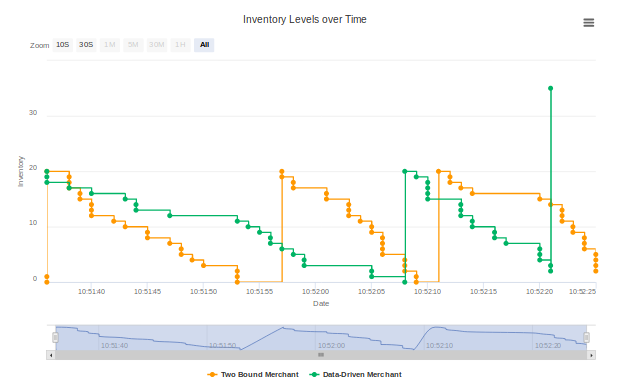
\includegraphics[width=0.8\textwidth]{figures/inventory_graph}
	\caption[Inventory Chart on the \UI]{Example of the Inventory Chart in the \ui showing inventory levels over time of two competing merchants.}
	\label{fig:invnetory_graph}
\end{figure}

%more motivation?
The platform extensions create the inventory control problem for merchants.
Merchants' inventory levels are more important than ever before because of this problem.
In order to analyze how merchants control their inventory levels, we added an inventory chart to the \ui.
Users have access to the new chart that shows inventory levels over time from all merchants.
\cref{fig:invnetory_graph} shows an example of the inventory chart.
This chart is shown along other charts, which present metrics like prices, profit, and revenue. 
We used the highcharts\footnote{JavaScript chart library, Highcharts: \url{https://www.highcharts.com/}} library to have the same look and feel as the existing charts.

\section{Benchmarking Tool}
\label{section:benchmark_tool}
%problem
Getting comparable results over multiple simulations on the \pricewars platform was problematic while developing our merchant.
The charts on the \ui are helpful in evaluating a single simulation run but it is not precise enough to compare multiple runs.
It is not feasible to manually examine charts at an exact timing.
A better way to compare simulation runs with each other is especially important in monopoly scenarios, when merchant with different configurations or strategies are compared.

%solution
We developed a benchmarking tool that runs simulations on the \pricewars platform with specified merchants for a certain duration.
This tool allows the user to run multiple simulations for the same duration.
With this tools, it is no longer necessary to read a chart at the right point in time.

After a run, the benchmark tool saves all events that happened on the platform from the event log.
The events contain orders, sales, and inventory levels among others and are saved in JSON format.
Events are analyzed to determine each merchant's profit, revenue, and expenses as shown in \cref{tab:benchmark_tool}.
These results are saves as a table in CSV format.

After a simulation, users can run additional analysis on the saved events to answer new questions, like: how many stock-outs had each merchant?
Another benefit from using the benchmark tool is the automated setup and teardown of the platform.
This process would need some manual steps otherwise like clearing the state from the previous simulation and starting the consumer.

\begin{table}[t]
	\centering
	\begin{tabular}{ lrrrr }
		\toprule
		\textbf{Merchant} & \textbf{Profit} & \textbf{Revenue} & \textbf{Holding Cost} & \textbf{Order Cost} \\
		\midrule
		Merchant A & 534.17 & 3\,547.00 & 212.83 & 2\,800.00 \\
		Merchant B & 315.12 & 4\,063.80 & 363.80 & 3\,385.00 \\
		Merchant C & 492.50 & 3\,844.80 & 152.30 & 3\,200.00 \\
		\bottomrule
	\end{tabular}
	\caption[Benchmark Tool: Breakdown of Expenses and Revenues]{The benchmark tool generates a breakdown of expenses and revenues. Results are shown from a five minute simulation.}
	\label{tab:benchmark_tool}
\end{table}

The benchmark tool is a Python script.
The command to run the tool is \texttt{python3 helper\_scripts/benchmark.py}.
The parameter \texttt{-{}-duration} controls the length of the simulation in minutes.
The user provides a list of merchant start commands to \texttt{-{}-merchants}.
The start commands are the same commands that would be used to start merchants manually.
The parameter \texttt{-{}-holding\_cost} sets the same holding cost rate for all merchants. 
Results are written to the directory given to the \texttt{-{}-output} parameter.
